% Created by tikzDevice version 0.12 on 2019-03-30 13:33:50
% !TEX encoding = UTF-8 Unicode
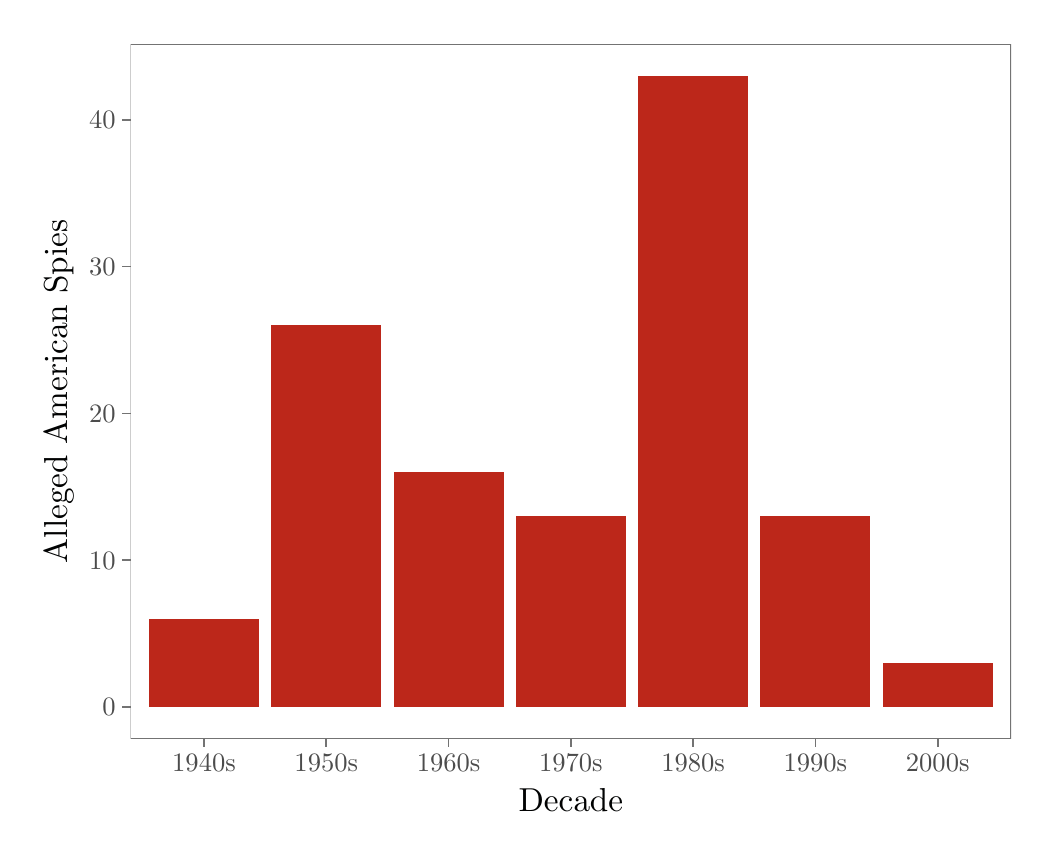
\begin{tikzpicture}[x=1pt,y=1pt]
\definecolor{fillColor}{RGB}{255,255,255}
\path[use as bounding box,fill=fillColor,fill opacity=0.00] (0,0) rectangle (361.35,289.08);
\begin{scope}
\path[clip] (  0.00,  0.00) rectangle (361.35,289.08);
\definecolor{drawColor}{RGB}{255,255,255}
\definecolor{fillColor}{RGB}{255,255,255}

\path[draw=drawColor,line width= 0.6pt,line join=round,line cap=round,fill=fillColor] (  0.00,  0.00) rectangle (361.35,289.08);
\end{scope}
\begin{scope}
\path[clip] ( 37.21, 32.28) rectangle (355.35,283.08);
\definecolor{fillColor}{RGB}{255,255,255}

\path[fill=fillColor] ( 37.21, 32.28) rectangle (355.35,283.08);
\definecolor{fillColor}{RGB}{188,39,26}

\path[fill=fillColor] ( 43.83, 43.68) rectangle ( 83.60, 75.49);

\path[fill=fillColor] ( 88.02, 43.68) rectangle (127.79,181.54);

\path[fill=fillColor] (132.21, 43.68) rectangle (171.98,128.51);

\path[fill=fillColor] (176.39, 43.68) rectangle (216.16,112.61);

\path[fill=fillColor] (220.58, 43.68) rectangle (260.35,271.68);

\path[fill=fillColor] (264.77, 43.68) rectangle (304.54,112.61);

\path[fill=fillColor] (308.95, 43.68) rectangle (348.72, 59.58);
\definecolor{drawColor}{gray}{0.45}

\path[draw=drawColor,line width= 0.6pt,line join=round,line cap=round] ( 37.21, 32.28) rectangle (355.35,283.08);
\end{scope}
\begin{scope}
\path[clip] (  0.00,  0.00) rectangle (361.35,289.08);
\definecolor{drawColor}{gray}{0.30}

\node[text=drawColor,anchor=base east,inner sep=0pt, outer sep=0pt, scale=  0.96] at ( 31.81, 40.37) {0};

\node[text=drawColor,anchor=base east,inner sep=0pt, outer sep=0pt, scale=  0.96] at ( 31.81, 93.39) {10};

\node[text=drawColor,anchor=base east,inner sep=0pt, outer sep=0pt, scale=  0.96] at ( 31.81,146.42) {20};

\node[text=drawColor,anchor=base east,inner sep=0pt, outer sep=0pt, scale=  0.96] at ( 31.81,199.44) {30};

\node[text=drawColor,anchor=base east,inner sep=0pt, outer sep=0pt, scale=  0.96] at ( 31.81,252.47) {40};
\end{scope}
\begin{scope}
\path[clip] (  0.00,  0.00) rectangle (361.35,289.08);
\definecolor{drawColor}{gray}{0.45}

\path[draw=drawColor,line width= 0.6pt,line join=round] ( 34.21, 43.68) --
	( 37.21, 43.68);

\path[draw=drawColor,line width= 0.6pt,line join=round] ( 34.21, 96.70) --
	( 37.21, 96.70);

\path[draw=drawColor,line width= 0.6pt,line join=round] ( 34.21,149.72) --
	( 37.21,149.72);

\path[draw=drawColor,line width= 0.6pt,line join=round] ( 34.21,202.75) --
	( 37.21,202.75);

\path[draw=drawColor,line width= 0.6pt,line join=round] ( 34.21,255.77) --
	( 37.21,255.77);
\end{scope}
\begin{scope}
\path[clip] (  0.00,  0.00) rectangle (361.35,289.08);
\definecolor{drawColor}{gray}{0.45}

\path[draw=drawColor,line width= 0.6pt,line join=round] ( 63.72, 29.28) --
	( 63.72, 32.28);

\path[draw=drawColor,line width= 0.6pt,line join=round] (107.90, 29.28) --
	(107.90, 32.28);

\path[draw=drawColor,line width= 0.6pt,line join=round] (152.09, 29.28) --
	(152.09, 32.28);

\path[draw=drawColor,line width= 0.6pt,line join=round] (196.28, 29.28) --
	(196.28, 32.28);

\path[draw=drawColor,line width= 0.6pt,line join=round] (240.46, 29.28) --
	(240.46, 32.28);

\path[draw=drawColor,line width= 0.6pt,line join=round] (284.65, 29.28) --
	(284.65, 32.28);

\path[draw=drawColor,line width= 0.6pt,line join=round] (328.84, 29.28) --
	(328.84, 32.28);
\end{scope}
\begin{scope}
\path[clip] (  0.00,  0.00) rectangle (361.35,289.08);
\definecolor{drawColor}{gray}{0.30}

\node[text=drawColor,anchor=base,inner sep=0pt, outer sep=0pt, scale=  0.96] at ( 63.72, 20.26) {1940s};

\node[text=drawColor,anchor=base,inner sep=0pt, outer sep=0pt, scale=  0.96] at (107.90, 20.26) {1950s};

\node[text=drawColor,anchor=base,inner sep=0pt, outer sep=0pt, scale=  0.96] at (152.09, 20.26) {1960s};

\node[text=drawColor,anchor=base,inner sep=0pt, outer sep=0pt, scale=  0.96] at (196.28, 20.26) {1970s};

\node[text=drawColor,anchor=base,inner sep=0pt, outer sep=0pt, scale=  0.96] at (240.46, 20.26) {1980s};

\node[text=drawColor,anchor=base,inner sep=0pt, outer sep=0pt, scale=  0.96] at (284.65, 20.26) {1990s};

\node[text=drawColor,anchor=base,inner sep=0pt, outer sep=0pt, scale=  0.96] at (328.84, 20.26) {2000s};
\end{scope}
\begin{scope}
\path[clip] (  0.00,  0.00) rectangle (361.35,289.08);
\definecolor{drawColor}{RGB}{1,2,2}

\node[text=drawColor,anchor=base,inner sep=0pt, outer sep=0pt, scale=  1.20] at (196.28,  6.00) {Decade};
\end{scope}
\begin{scope}
\path[clip] (  0.00,  0.00) rectangle (361.35,289.08);
\definecolor{drawColor}{RGB}{1,2,2}

\node[text=drawColor,rotate= 90.00,anchor=base,inner sep=0pt, outer sep=0pt, scale=  1.20] at ( 14.26,157.68) {Alleged American Spies};
\end{scope}
\end{tikzpicture}
